% - Sicherheits-Applikation/ Spezielle Firewall
% - Gefordert in diversen Compliance Richtlinien
% - Fokus auf web-Protokolle
%     - auf TCP/IP Layer 5
%     - HTTP, HTTPS, FTP
% - Traffic Analyse in Tiefe (Request & Response)
%     - HTTP (kapitel 5.2) beschreibt diverse Angriffswege
%     - Erkennung anhand von Regeln
%         - Black- vs. whitelisting
%         - Vordefiniertes Regelwerk
\label{chap:waf-theory}

Mit dem Namen \ac{waf} wird eine Sicherheits-Anwendung beschrieben, die in der Lage ist den Datenverkehr zu und von einer Webanwendung zu analysieren und auf Sicherheitskritische Inhalte zu überprüfen. 
Eine \ac{waf} ist hierbei in der Lage gefährliche Inhalte nicht nur zu blockieren, sondern anfragen auch so zu verändern, dass sie unschädlich sind und trotzdem verarbeitet werden können.
Im Gegensatz zu einer \textit{klassischen} Firewall, die auf den Schichten 3 und 4 des OSI/ISO Schichten-Modells arbeitet, ist eine \ac{waf} in der Lage passierenden Datenverkehr auf der Anwendungsschicht (Schicht 7) zu analysieren. 
Hierbei liegt der Fokus hauptsächlich auf dem \ac{http}. Es ist jedoch auch möglich andere, im Kontext von Webanwendungen genutzte Protokolle wie FTP zu analysieren.
Um des gesamten Inhalt der zu analysierenden Nachrichten sehen zu können (Deep Packet Inspection) kann eine \ac{waf} Protokolle zur Sicherstellung von Vertraulichkeit und Integrität (SSL/TLS) terminieren.
\\
Es gibt mehrere kommerzielle Hersteller aber auch Opern-Source Entwickler die \acp{waf} zur Verfügung stellen.
Diese Angebote können auf eine vielzahl von Wegen logisch vor einer Webanwendung positioniert werden.
Während große Hosting- und Serveranbieter wie Cloudflare or Microsoft azure es ermöglichen mittels wenigen kicks eine \ac{waf} vor die bei ihnen untergebrachten webserver zu installieren, können die Angebote anderer, eigenständiger \acp{waf} auf unterschiedliche Methoden betrieben werden:
\begin{enumerate}
     \item Als physischer Server in einem Rechenzentrum
     \item Als Eigenständige virtuelle Maschine innerhalb der eingenen Virtualisierungsumgebung
     \item Als Einheit in einer Containervirtualisierungsumgebung
     \item Als Modul oder Addon einer Webserver-Anwendung (NGINX/Apache webserver)
\end{enumerate}

Daraus ergeben sich zwei gängige Deployment Szenarien.

\begin{itemize}
     \item \textit{On premise Deployment} bei dem sich die \ac{waf} neben den zu schützenden Anwendungen im gleichen Netzwerk befindet
     \item \textit{Cloud WAF} wo die \ac{waf} von einem Drittanbieter zur Verfügung Gestellt wird und mittels IP-Whitelisting sichergestellt werden muss, dass ein zugriff auf die Webanwendung nur durch die \ac{waf} erfolgen kann.
\end{itemize}
Der Betrieb einer \ac{waf} erfordert die Anpassung an die zu schützende Anwendung. Es muss eine Konfiguration sichergestellt werden, dass die Funktion einer Webanwendung nicht beeinträchtigt ist ohne dabei die schützenden Funktion der \ac{waf} einzuschränken.

Um abgrenzen zu können welche Inhalte für Lerninhalte in Frage kommen und abzuschätzen was in der vorgegeben Zeit vermittelt werden kann wird im folgenden Kapitel eine \ac{waf} detailliert beschrieben.

\subsubsection{Verarbeitung einer Anfrage}
\paragraph{Request Parsing}
% - SSL Termination
% - HTTP/HTTPS Parsing
% - Nachsichten Felder extrahieren
% - Anfragen Normalisierung
% - Überführen in ein standardisiertes Format
% - Gegen diverse evasion techniken
%     - null byte
%     - self-referencing directories
%     - path traversals
%     - URL encoding

\begin{figure}[!hbt]
    \centering
    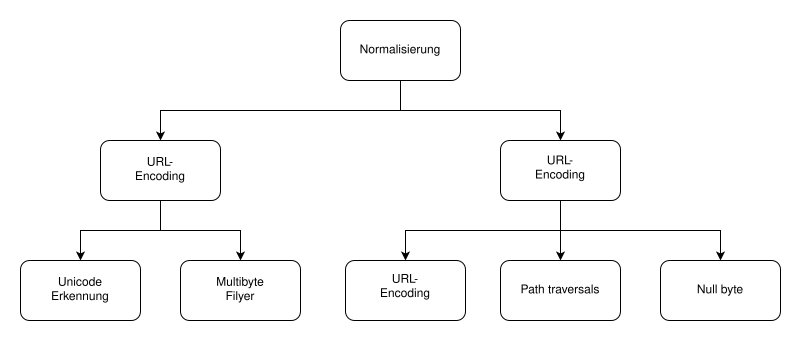
\includegraphics[width=0.9\textwidth]{./images/Normalisierung.png}
    \caption{Normalisierungs-Schritte}
    \label{fig:norming}
\end{figure}


\paragraph{Muster-Abgleich gegen Regeln}
% - Abgleichen gegen Feature Datenbank
% - Jeder Parameter gegen jede regex
%     - Rechenaufwand
%         - optimierte regex-Engines
%         - Tree pruning
%             - Gefahr durch ungewollte pass on Szenarien
% - Whitelisting
%     - Features deaktivieren die web app-Funktion einschränken
% - Blacklisting
%     - Default Regelwerk
% - Auch Signatur-basierte WAFs
%     - komplexere Erkennung

\paragraph{Logging}
% - Jeder Schritt wird protokolliert
%     - Compliance
%         - Erfiltrierte Daten
%         - betroffene Nutzer
%     - Nachvollziehbarkeit von Fehlern
% - Log analyse
%     - Hauptarbeit eines WAF-Consultants

\paragraph{Weiteres Vorgehen}
% - Request Ablehnen
%     - Werden schädliche Daten erkannt
% - Request modifizieren
%     - Ablehnen bei schädlichen Inhalten nicht notwendig
%     - request kann umgeschrieben werden
%         - Abschnitte entfernen
%         - Abschnitte Escapeen
% - unmodofiziertes weiterleiten
% 
% - aus normalisierter form HTTP-Request erstellen
% - an server übergeben

\subsubsection{Erweiterte Funktionen}
\paragraph{Lernen von Regeln aus vorhergegangenem Datenverkehr}
\paragraph{KI-Features}
\subsubsection{Deployment einer WAF}
\paragraph{Postitionierung einer WAF}
\paragraph{Betrieb einer WAF}
\subsubsection{Schwächen und Nachteile einer WAF}
